\documentclass[journal,12pt,twocolumn]{IEEEtran}
%\usepackage{setspace}
\usepackage{gensymb}
%\doublespacing
%\singlespacing

%\usepackage{graphicx}
%\usepackage{amssymb}
%\usepackage{relsize}
\usepackage[cmex10]{amsmath}
%\usepackage{amsthm}
%\interdisplaylinepenalty=2500
%\savesymbol{iint}
%\usepackage{txfonts}
%\restoresymbol{TXF}{iint}
%\usepackage{wasysym}
\usepackage{amsthm}
%\usepackage{iithtlc}
\usepackage{mathrsfs}
\usepackage{txfonts}
\usepackage{stfloats}
\usepackage{bm}
\usepackage{cite}
\usepackage{cases}
\usepackage{subfig}
%\usepackage{xtab}
\usepackage{longtable}
\usepackage{multirow}
%\usepackage{algorithm}
%\usepackage{algpseudocode}
\usepackage{enumitem}
\usepackage{mathtools}
\usepackage{tikz}
\usepackage{circuitikz}
\usepackage{verbatim}
%\usepackage{tfrupee}
%\usepackage[breaklinks=true]{hyperref}
%\usepackage{stmaryrd}
%\usepackage{tkz-euclide} % loads  TikZ and tkz-base
%\usetkzobj{all}
%\usepackage{listings}
    \usepackage{color}                                            %%
    \usepackage{array}                                            %%
    \usepackage{longtable}                                        %%
    \usepackage{calc}                                             %%
    \usepackage{multirow}                                         %%
    \usepackage{hhline}                                           %%
    \usepackage{ifthen}                                           %%
  %optionally (for landscape tables embedded in another document): %%
    \usepackage{lscape}     
\usepackage{multicol}
\usepackage{chngcntr}
%\usepackage{enumerate}

%\usepackage{wasysym}
%\newcounter{MYtempeqncnt}
\DeclareMathOperator*{\Res}{Res}
%\renewcommand{\baselinestretch}{2}
\renewcommand\thesection{\arabic{section}}
\renewcommand\thesubsection{\thesection.\arabic{subsection}}
\renewcommand\thesubsubsection{\thesubsection.\arabic{subsubsection}}

\renewcommand\thesectiondis{\arabic{section}}
\renewcommand\thesubsectiondis{\thesectiondis.\arabic{subsection}}
\renewcommand\thesubsubsectiondis{\thesubsectiondis.\arabic{subsubsection}}

% correct bad hyphenation here
\hyphenation{op-tical net-works semi-conduc-tor}
\def\inputGnumericTable{}                                 %%

%\lstset{
%language=C,
%frame=single, 
%breaklines=true,
%columns=fullflexible
%}
%\lstset{
%language=tex,
%frame=single, 
%breaklines=true
%}

\begin{document}
%


\newtheorem{theorem}{Theorem}[section]
\newtheorem{problem}{Problem}
\newtheorem{proposition}{Proposition}[section]
\newtheorem{lemma}{Lemma}[section]
\newtheorem{corollary}[theorem]{Corollary}
\newtheorem{example}{Example}[section]
\newtheorem{definition}[problem]{Definition}
%\newtheorem{thm}{Theorem}[section] 
%\newtheorem{defn}[thm]{Definition}
%\newtheorem{algorithm}{Algorithm}[section]
%\newtheorem{cor}{Corollary}
\newcommand{\BEQA}{\begin{eqnarray}}
\newcommand{\EEQA}{\end{eqnarray}}
\newcommand{\define}{\stackrel{\triangle}{=}}
\bibliographystyle{IEEEtran}
%\bibliographystyle{ieeetr}
\providecommand{\mbf}{\mathbf}
\providecommand{\pr}[1]{\ensuremath{\Pr\left(#1\right)}}
\providecommand{\qfunc}[1]{\ensuremath{Q\left(#1\right)}}
\providecommand{\sbrak}[1]{\ensuremath{{}\left[#1\right]}}
\providecommand{\lsbrak}[1]{\ensuremath{{}\left[#1\right.}}
\providecommand{\rsbrak}[1]{\ensuremath{{}\left.#1\right]}}
\providecommand{\brak}[1]{\ensuremath{\left(#1\right)}}
\providecommand{\lbrak}[1]{\ensuremath{\left(#1\right.}}
\providecommand{\rbrak}[1]{\ensuremath{\left.#1\right)}}
\providecommand{\cbrak}[1]{\ensuremath{\left\{#1\right\}}}
\providecommand{\lcbrak}[1]{\ensuremath{\left\{#1\right.}}
\providecommand{\rcbrak}[1]{\ensuremath{\left.#1\right\}}}
\theoremstyle{remark}
\newtheorem{rem}{Remark}
\newcommand{\sgn}{\mathop{\mathrm{sgn}}}
\providecommand{\abs}[1]{\left\vert#1\right\vert}
\providecommand{\res}[1]{\Res\displaylimits_{#1}} 
\providecommand{\norm}[1]{\left\lVert#1\right\rVert}
%\providecommand{\norm}[1]{\lVert#1\rVert}
\providecommand{\mtx}[1]{\mathbf{#1}}
\providecommand{\mean}[1]{E\left[ #1 \right]}
\providecommand{\fourier}{\overset{\mathcal{F}}{ \rightleftharpoons}}
%\providecommand{\hilbert}{\overset{\mathcal{H}}{ \rightleftharpoons}}
\providecommand{\system}{\overset{\mathcal{H}}{ \longleftrightarrow}}
	%\newcommand{\solution}[2]{\textbf{Solution:}{#1}}
\newcommand{\solution}{\noindent \textbf{Solution: }}
\newcommand{\cosec}{\,\text{cosec}\,}
\providecommand{\dec}[2]{\ensuremath{\overset{#1}{\underset{#2}{\gtrless}}}}
\newcommand{\myvec}[1]{\ensuremath{\begin{pmatrix}#1\end{pmatrix}}}
\newcommand{\mydet}[1]{\ensuremath{\begin{vmatrix}#1\end{vmatrix}}}
%\numberwithin{equation}{section}
\numberwithin{equation}{subsection}
%\numberwithin{problem}{section}
%\numberwithin{definition}{section}
\makeatletter
\@addtoreset{figure}{problem}
\makeatother
\let\StandardTheFigure\thefigure
\let\vec\mathbf
%\renewcommand{\thefigure}{\theproblem.\arabic{figure}}
\renewcommand{\thefigure}{\theproblem}
%\setlist[enumerate,1]{before=\renewcommand\theequation{\theenumi.\arabic{equation}}
%\counterwithin{equation}{enumi}
%\renewcommand{\theequation}{\arabic{subsection}.\arabic{equation}}
\def\putbox#1#2#3{\makebox[0in][l]{\makebox[#1][l]{}\raisebox{\baselineskip}[0in][0in]{\raisebox{#2}[0in][0in]{#3}}}}
     \def\rightbox#1{\makebox[0in][r]{#1}}
     \def\centbox#1{\makebox[0in]{#1}}
     \def\topbox#1{\raisebox{-\baselineskip}[0in][0in]{#1}}
     \def\midbox#1{\raisebox{-0.5\baselineskip}[0in][0in]{#1}}
\vspace{3cm}
\title{
	\logo{
Control Systems
	}
}
\author{ G V V Sharma$^{*}$% <-this % stops a space
	\thanks{*The author is with the Department
		of Electrical Engineering, Indian Institute of Technology, Hyderabad
		502285 India e-mail:  gadepall@iith.ac.in. All content in this manual is released under GNU GPL.  Free and open source.}
	
}	
%\title{
%	\logo{Matrix Analysis through Octave}{\begin{center}\includegraphics[scale=.24]{tlc}\end{center}}{}{HAMDSP}
%}
% paper title
% can use linebreaks \\ within to get better formatting as desired
%\title{Matrix Analysis through Octave}
%
%
% author names and IEEE memberships
% note positions of commas and nonbreaking spaces ( ~ ) LaTeX will not break
% a structure at a ~ so this keeps an author's name from being broken across
% two lines.
% use \thanks{} to gain access to the first footnote area
% a separate \thanks must be used for each paragraph as LaTeX2e's \thanks
% was not built to handle multiple paragraphs
%
%\author{<-this % stops a space
%\thanks{}}
%}
% note the % following the last \IEEEmembership and also \thanks - 
% these prevent an unwanted space from occurring between the last author name
% and the end of the author line. i.e., if you had this:
% 
% \author{....lastname \thanks{...} \thanks{...} }
%                     ^------------^------------^----Do not want these spaces!
%
% a space would be appended to the last name and could cause every name on that
% line to be shifted left slightly. This is one of those "LaTeX things". For
% instance, "\textbf{A} \textbf{B}" will typeset as "A B" not "AB". To get
% "AB" then you have to do: "\textbf{A}\textbf{B}"
% \thanks is no different in this regard, so shield the last } of each \thanks
% that ends a line with a % and do not let a space in before the next \thanks.
% Spaces after \IEEEmembership other than the last one are OK (and needed) as
% you are supposed to have spaces between the names. For what it is worth,
% this is a minor point as most people would not even notice if the said evil
% space somehow managed to creep in.
% The paper headers
%\markboth{Journal of \LaTeX\ Class Files,~Vol.~6, No.~1, January~2007}%
%{Shell \MakeLowercase{\textit{et al.}}: Bare Demo of IEEEtran.cls for Journals}
% The only time the second header will appear is for the odd numbered pages
% after the title page when using the twoside option.
% 
% *** Note that you probably will NOT want to include the author's ***
% *** name in the headers of peer review papers.                   ***
% You can use \ifCLASSOPTIONpeerreview for conditional compilation here if
% you desire.
% If you want to put a publisher's ID mark on the page you can do it like
% this:
%\IEEEpubid{0000--0000/00\$00.00~\copyright~2007 IEEE}
% Remember, if you use this you must call \IEEEpubidadjcol in the second
% column for its text to clear the IEEEpubid mark.
% make the title area
%\maketitle
\newpage
\tableofcontents
\bigskip
\renewcommand{\thefigure}{\theenumi}
\renewcommand{\thetable}{\theenumi}
%\renewcommand{\theequation}{\theenumi}
%\begin{abstract}
%%\boldmath
%In this letter, an algorithm for evaluating the exact analytical bit error rate  (BER)  for the piecewise linear (PL) combiner for  multiple relays is presented. Previous results were available only for upto three relays. The algorithm is unique in the sense that  the actual mathematical expressions, that are prohibitively large, need not be explicitly obtained. The diversity gain due to multiple relays is shown through plots of the analytical BER, well supported by simulations. 
%
%\end{abstract}
% IEEEtran.cls defaults to using nonbold math in the Abstract.
% This preserves the distinction between vectors and scalars. However,
% if the journal you are submitting to favors bold math in the abstract,
% then you can use LaTeX's standard command \boldmath at the very start
% of the abstract to achieve this. Many IEEE journals frown on math
% in the abstract anyway.
% Note that keywords are not normally used for peerreview papers.
%\begin{IEEEkeywords}
%Cooperative diversity, decode and forward, piecewise linear
%\end{IEEEkeywords}
% For peer review papers, you can put extra information on the cover
% page as needed:
% \ifCLASSOPTIONpeerreview
% \begin{center} \bfseries EDICS Category: 3-BBND \end{center}
% \fi
%
% For peerreview papers, this IEEEtran command inserts a page break and
% creates the second title. It will be ignored for other modes.
%\IEEEpeerreviewmaketitle
\begin{abstract}
This manual is an introduction to control systems based on GATE problems.Links to sample Python codes are available in the text.  
\end{abstract}
Download python codes using 
%\begin{lstlisting}
%svn co https://github.com/gadepall/school/trunk/control/codes
%\end{lstlisting}
%\section{Bode Plot}
%\begin{enumerate}[label=\thesection.\arabic*.,ref=\thesection.\theenumi]
%\numberwithin{equation}{enumi}
%\input{./chapters/ee18btech11001.tex}
%\end{enumerate}
\section{Stability}
\subsection{Second order System}
\section{Routh Hurwitz Criterion}
\section{Compensators}
\section{Nyquist Plot}
%\section{Triangle}
%\subsection{Triangle Examples}
%\input{./triangle/tri_exam.tex} 
%\subsection{Triangle Exercises}
%\input{./triangle/tri_geo.tex} 
%%
%\section{Quadrilateral}
%\subsection{Quadrilateral Examples}
%\input{./quad/quad_geo_exam.tex} 
%\subsection{Quadrilateral Geometry}
%\input{./quad/quad_geo.tex} 
%
%\section{Constrained Optimization}
%%\subsection{Equality Constraint}
%\input{./chapters/line_exam.tex}
%\section{Convex Function}
%\input{./chapters/conv.tex}
%\section{Gradient Descent}
%\input{./chapters/grad_des.tex}
%\section{Lagrange Multipliers}
%\input{./chapters/lagrange.tex}
%\section{Quadratic Programming}
%\input{./chapters/qp.tex}
%\section{Semi Definite Programming}
%\input{./chapters/sdp.tex}
%\section{Linear Programming}
%\input{./chapters/lp_exam.tex}
%\section{Exercises}
\begin{enumerate}[label=\thesection.\arabic*.,ref=\thesection.\theenumi]
\numberwithin{equation}{enumi}
\item Which of the following is \textbf{incorrect} ?\\
(A) Lead compensator is used to reduce the settling time\\
(B) Lag compensator is used to reduce the steady state error\\
(C) Lead compensator may increase the order of a system\\
(D) Lag compensator always stabilzes an unstable system\\
\\
\solution 
\begin{figure}[h]
\begin{center}
\resizebox{\columnwidth}{!}{\tikzstyle{block} = [draw, fill=blue!20, rectangle, 
    minimum height=0.7cm, minimum width=0.7cm]
\tikzstyle{sum} = [draw, fill=blue!20, circle, node distance=1cm]
\tikzstyle{input} = [coordinate]
\tikzstyle{output} = [coordinate]
\tikzstyle{pinstyle} = [pin edge={to-,thin,black}]

\begin{tikzpicture}[auto, node distance=2.5cm,>=latex']
    % We start by placing the blocks
    \node [input, name=input] {};
    %\node [sum, right of=input] (sum) {};
    \node [block, right of=input] (controller) {G(s)};
    \node [output, right of=controller] (output) {};


    \draw [draw,->] (input) -- node {$R(s)$} (controller);
    %\draw [->] (sum) -- node {$E(s)$} (controller);
    \draw [->] (controller) -- node [name=y] {$Y(s)$}(output);
   % \draw [->] (y) -- ++ (0,-2) -| node [pos=0.99] {$-$} (sum);
 
\end{tikzpicture}}
\end{center}
\end{figure}
\\
Statement - A\\Lead compensator is used to reduce settling time.
\begin{align}
system-G(s) = \frac{1}{s(3s+1)}\\
lead\ compensator-D(s) = \frac{3(s+\frac{1}{3})}{(s+1)} \\
hence, new\ system-G_{1}(s) = \frac{1}{s(s+1)}
\end{align}
\\
\textbf{unit impulse response}\\
without lead compensator - \\
\begin{align}
G(s) = \frac{1}{(s)(3s+1)}\\
Y(s) = G(s).1\\
Y(s) = \frac{1}{(s)(3s+1)}
\end{align}
splitting into partial fractions\\
\begin{align}
Y(s) = \frac{1}{s} - \frac{1}{s+\frac{1}{3}}
\end{align}
taking inverse laplace transform, \\
\begin{align}
y(t) = [ 1 - e^{\frac{-t}{3}}]u(t)
\end{align}
\\
with lead compensator - \\
\begin{align}
G(s) = \frac{1}{(s)(3s+1)}\\
D(s) = \frac{3(s+\frac{1}{3})}{(s+1)} \\
G_{1}(s) = \frac{1}{s(s+1)}\\
Y_{1}(s) = G_{1}(s).1\\
Y_{1}(s) = \frac{1}{s(s+1)}
\end{align}
splitting into partial fractions\\
\begin{align}
Y_{1}(s) = \frac{1}{s} - \frac{1}{s+1}
\end{align}
taking inverse laplace transform, \\
\begin{align}
y(t) = [ 1 - e^{-t}]u(t)
\end{align}
\\
\textbf{unit step response}
without lead compensator - \\
\begin{align}
G(s) = \frac{1}{(s)(3s+1)}\\
Y(s) = G(s).\frac{1}{s}\\
Y(S) = \frac{1}{(s^2)(3s+1)}
\end{align}
splitting into partial fractions\\
\begin{align}
Y(s) = \frac{1}{s^2} + \frac{3}{s+\frac{1}{3})} + \frac{-3}{s}
\end{align}
taking inverse laplace transform, \\
\begin{align}
y(t) = [t + 3e^{\frac{-t}{3}} - 3]u(t)
\end{align}
\\
with lead compensator - \\
\begin{align}
G(s) = \frac{1}{(s)(3s+1)}\\
D(s) = \frac{3(s+\frac{1}{3})}{(s+1)} \\
G_{1}(s) = \frac{1}{s(s+1)}\\
Y_{1}(s) = G_{1}(s).\frac{1}{s}\\
Y_{1}(s) = \frac{1}{(s^2)(s+1)}
\end{align}
splitting into partial fractions\\
\begin{align}
Y_{1}(s) = \frac{1}{s^2} + \frac{1}{s+1} - \frac{1}{s}
\end{align}
taking inverse laplace transform, \\
\begin{align}
y(t) = [t + e^{-t} - 1]u(t)
\end{align}
\\
\begin{figure}
\begin{subfigure}{\textwidth}
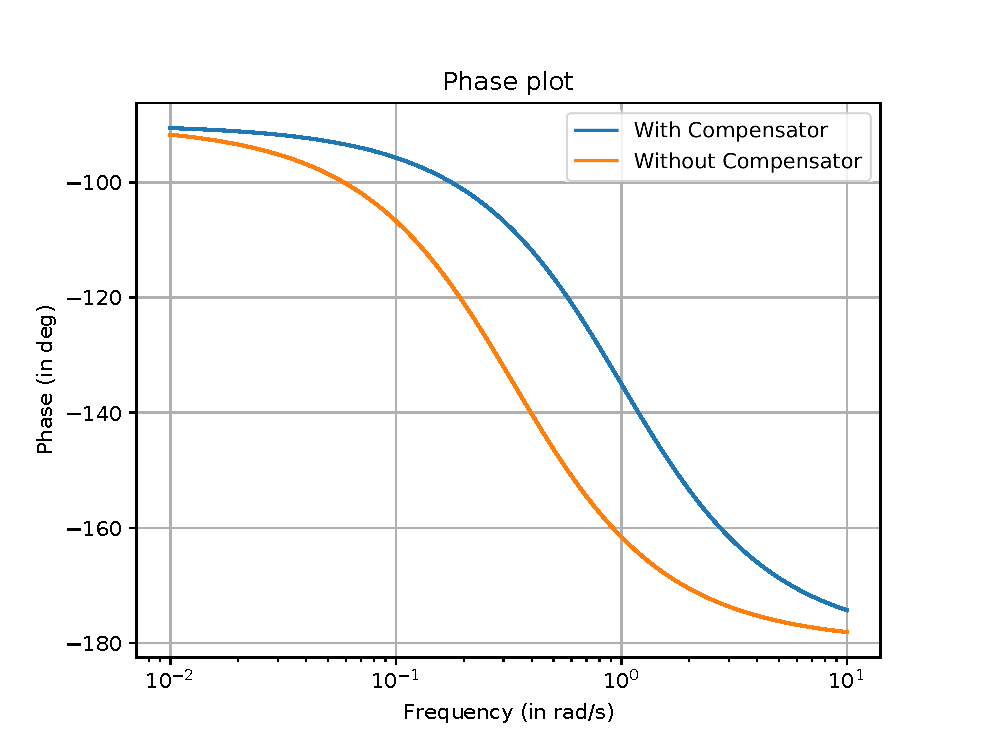
\includegraphics[width=1\linewidth, height=7cm ,inner]{./figs/ee18btech11027/lead_compensator_phase.eps} 
\label{fig:subim1}
\end{subfigure}
\end{figure}

\begin{figure}
\begin{subfigure}{\textwidth}
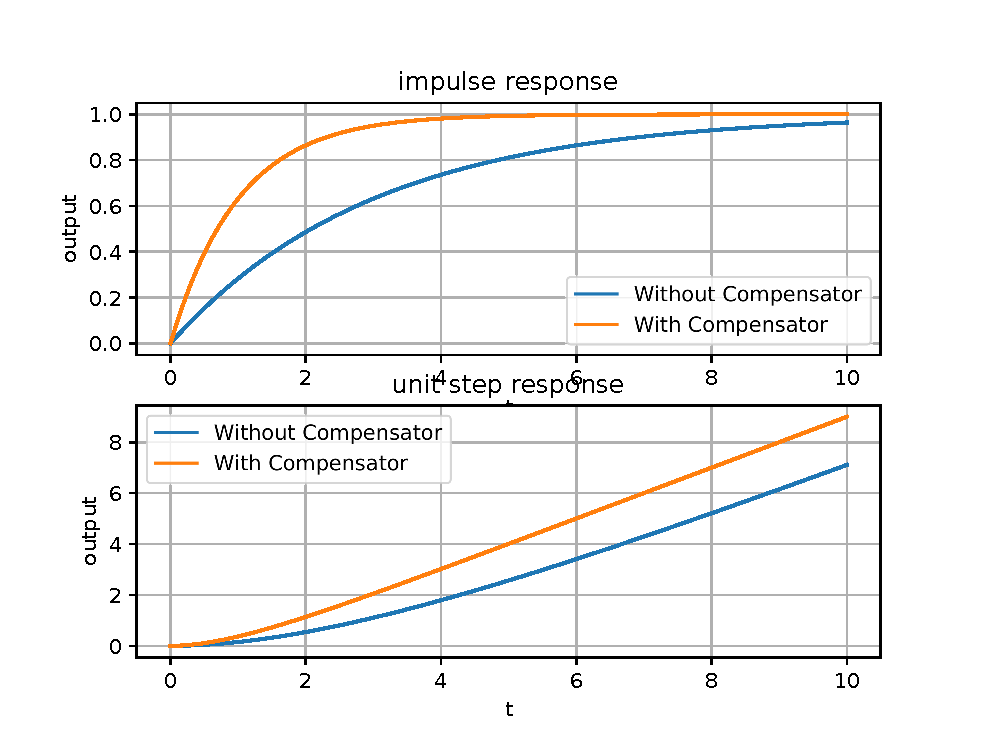
\includegraphics[width=1\linewidth, height=7cm ,inner]{./figs/ee18btech11027/settling_time.eps} 
\label{fig:subim1}
\end{subfigure}
\end{figure}
\\
Since lead compensator adds + phase for any value of frequency, the bode plot for phase vs frequency is above the one which is without lead compensator.\\

phase margin \phi_m = 180 + \phi_{gain = 0}\\
as\ lead\ compensator\ adds\ additional\ phase\ at\ all\\
frequencies, \\
$\phi_{gain = 0}$ \ gets increased, and hence\ phase\ margin

Relation between phase margin and damping ratio
Now,
\zeta = 0.01 $\times$ \phi_m\\

from this we get that damping factor also increases.\\

\implies damping\ is\ increased \\

\implies settling\ time\ decreased\\

Relation between phase margin and damping ratio.
Consider a second order system,\\
\begin{align}
G(s) = {\huge{$\frac{\omega_n^2}{s^2+2\zeta\omega_ns+\omega_n^2} $}}
\end{align}
 using value of $\phi_m$ to solve for $\zeta$.\\

set 20 $\log{|G(s)|}$ = -3dB to solve for \omega_n\\

using this equations we get,\\
\begin{align}
\phi_m = \tan^{-1}{\frac{2\zeta}{\sqrt{\sqrt{1+4\zeta^4} - 2\zeta^2}}}
\end{align}\\
a handy relation is - \zeta = 0.01\phi_m\\

\begin{figure}[h]
 
\begin{subfigure}{\textwidth}
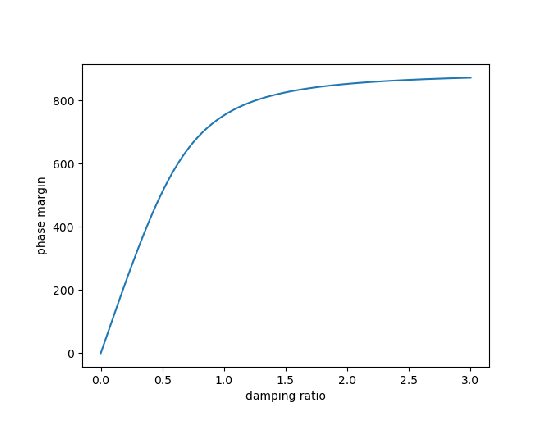
\includegraphics[width=1\linewidth, height=7cm ,inner]{./figs/ee18btech11027/realtion.eps} 
\label{fig:subim1}
\end{subfigure}
\end{figure}


 

    
Statement - B\\Lag compensator is used to reduce the steady state error.\\
Verification - 
Let the system transfer function be -
\begin{equation}
   c(s)= \frac{1}{s+2}
\end{equation}
and the lag compensator be- 
\begin{equation}
   t(s)= \frac{s+3}{s+1}
\end{equation}
therefore resulting system transfer function-
\begin{equation}
    G(s) = \frac{s+3}{(s+2)(s+1)}
\end{equation}

Hence steady state error for unit step input,\\

Without lag compensator = $\frac{1}{1+c(s)}$ \\

as s \to 0
\implies $E_{ss} = \frac{1}{1+0.5}$  \implies E_{ss} = 0.66\\

With lag compensator = $\frac{1}{1+G(s)}$\\

as s \to 0
{\implies} $E_{ss} = \frac{1}{1+1.5}$  \implies E_{ss} = 0.4\\

hence,\ the\ steady\ state\ error\ reduces.\\
\\
From\ the\ bode\ plot\ it\ is\ clear\ that\ the\ lag\ compensator\ has\ an\ high\ gain\ for\ low frequencies.\\
since steady state error is given by - 
\begin{align}
    e(\infty) = \lim_{s\to0} \frac{sR(s)}{1+G(s)}
\end{align}
\\
for low frequencies - the gain is high \implies G(s) \to large\ number\\in
{\implies e(\infty) \to smaller\ value\\}
{\implies steady\ state\ error\ decreases} \\
\begin{figure}[h]
 
\begin{subfigure}{\textwidth}
\includegraphics[width=1\linewidth, height=4cm ,inner]{./figs/ee18btech11027/table.eps} 
\label{fig:subim1}
\end{subfigure}
\end{figure}
\\
Statement - C\\Lead\ compensator\ may\ increase\ the\ order\ of\ a\ system.
\\
consider -

\begin{align}
G(s) = \frac{1}{s+2}\\
D(s) = \frac{s+1}{s+3}\\
G(s)\textbf{.}D(s) = \frac{s+1}{(s+2)(s+3)}\\
G(s)\textbf{.}D(s) = \frac{s+1}{s^2+5s+6}
\end{align}
\begin{flushleft}
Maximum power in denominator = 2\\
Hence order increased to 2 from 1\\
Lead compensator may increase the order of a system
since the transfer function adds a pole and a zero therefore it may increase the order of a system.\\
\end{flushleft}
\\
\\
\\
\\
\begin{flushleft}
Statement - D\\ Lag compensator always stabilizes an unstable system.
\begin{flushleft}
This statement is wrong.Consider,\\
\end{flushleft}
\begin{align}
G(s) = \frac{1}{s-2}\\
D(s) = \frac{s+3}{s+1}\\
G(s)\textbf{.}D(s) = \frac{(s+3)}{(s-2)(s+1)}\\ \\
output = 1.66e^{(2t)} + 0.66e^{(-t)}
\end{align}
\begin{flushleft}
If a system has a pole on right side of s plane, lag compensator cannot stabilize those systems. This is because the resulting system also has an pole on the right side of s plane.
\end{flushleft}


\textbf{}\begin{figure}[h]
 
\begin{subfigure}{\textwidth}
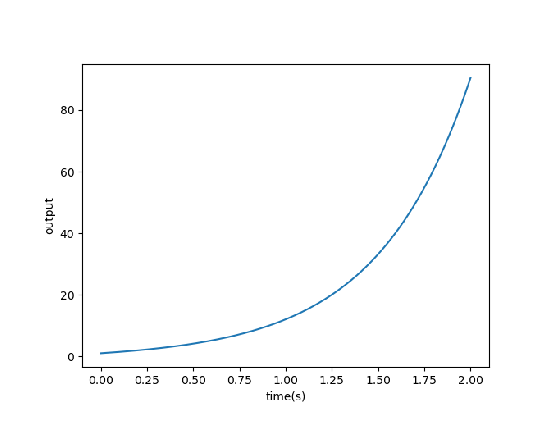
\includegraphics[width=1.05\linewidth, height=8cm ,inner]{./figs/ee18btech11027/unstable.eps} 
\label{fig:subim1}
\end{subfigure}
\end{figure}

\textbf{Lead and Lag compensators -}
\\
\\* \textbf{Lead compensator } - The lead compensator is an electrical network which produces a output having \textbf{phase lead} when a input is applied. 
\\
\begin{equation}
H(s) = \frac{s+z}{s+p}   0 \textless z \textless p
\centering
\end{equation}


 
The lead compensator circuit in the ‘s’ domain is shown in the following figure.
 
\begin{figure}[h]
 
\begin{subfigure}{0.5\textwidth}
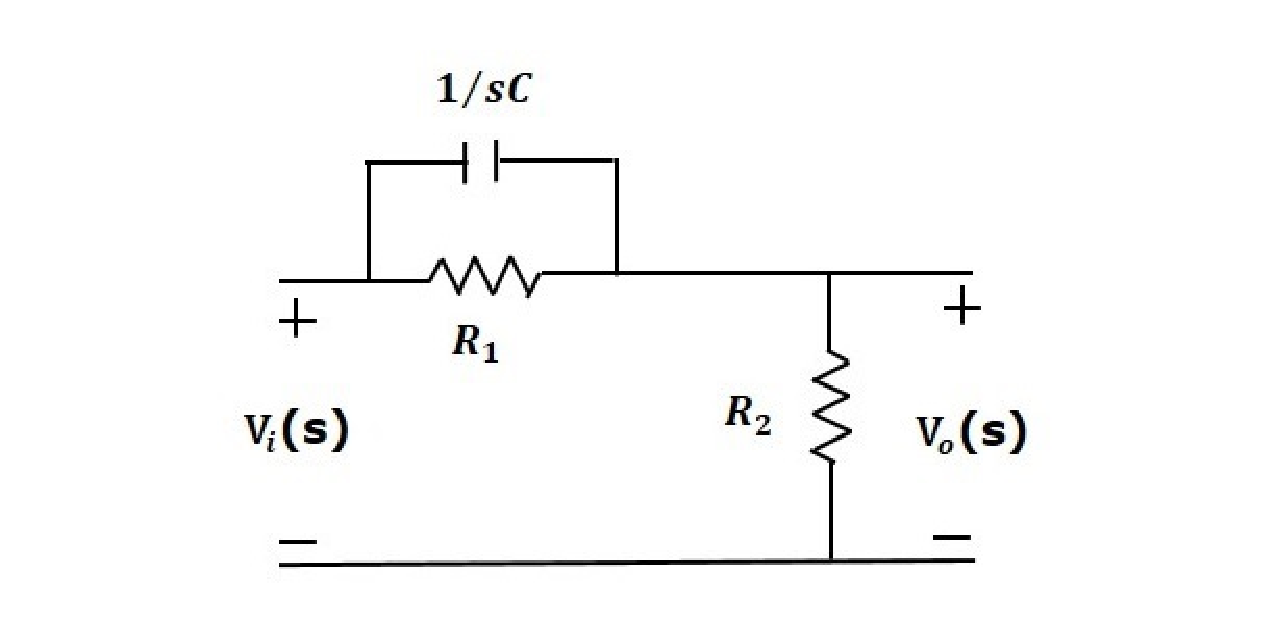
\includegraphics[width=0.9\linewidth, height=5cm ,inner]{./figs/ee18btech11027/lead_compensator.eps} 
\label{fig:subim1}
\end{subfigure}
\end{figure}


 
The transfer function of this lead compensator is -
\begin{align}
    \frac{V_o(s)}{V_i(s)} = \beta  \frac{s \tau +1}{s\beta \tau +1} \\
where\\
\tau = R_1C  \beta =\frac{R_2}{R_1+R_2}
\end{align}

\vspace{0.3cm}substituting s=j\omega, \ \frac{V_o(j\omega)}{V_i(j\omega)} = \beta  \frac{j\omega \tau +1}{j \omega\beta \tau +1}

\\
\begin{align}
phase angle \phi = \tan^{-1} {(\omega\tau)} - \tan{-1}{(\omega\beta\tau)}\\
since 0 \textless \ \beta < 1\\
\phi > 0
\end{align}

\\* \textbf{\\Lag compensator} - The Lag Compensator is an electrical network which produces a  output having the \textbf{phase lag} when a input is applied.
\begin{equation}
H(s) = \frac{s+z}{s+p}  \hspace{1cm} 0 \textless p \textless z
\centering
\end{equation}

 
The lag compensator circuit in the ‘s’ domain is shown in the following figure.
 
\begin{figure}[h]
 
\begin{subfigure}{0.5\textwidth}
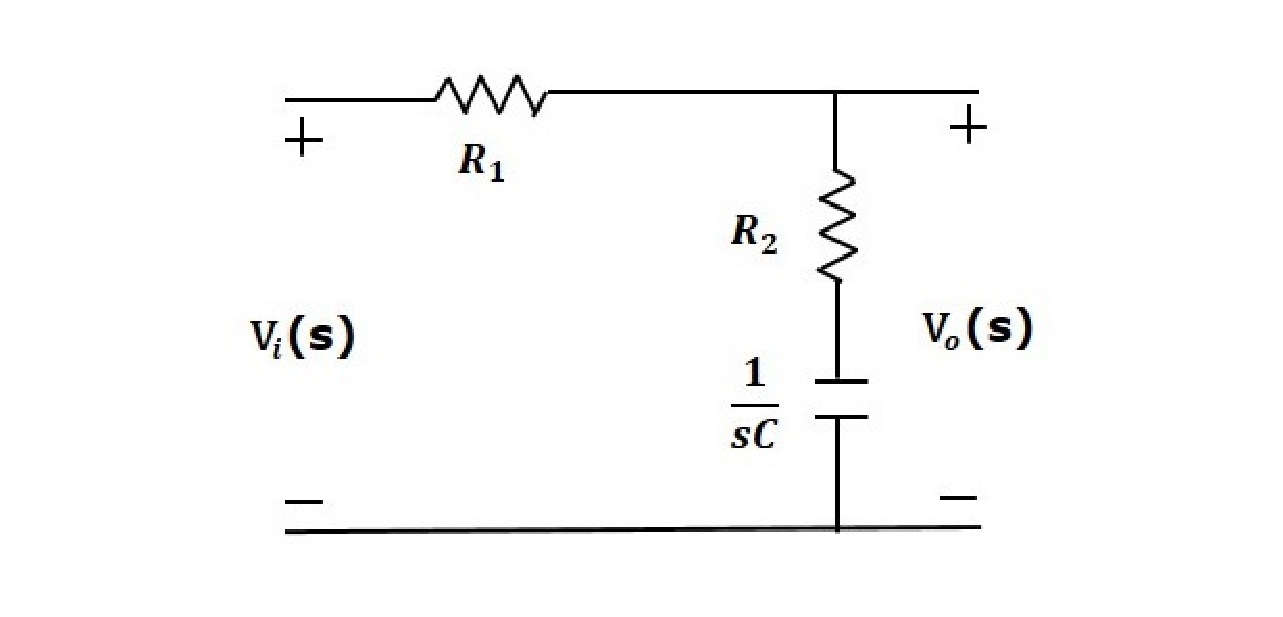
\includegraphics[width=0.9\linewidth, height=5cm ,inner]{./figs/ee18btech11027/lag_compensator.eps} 
\label{fig:subim1}
\end{subfigure}
\end{figure}
\\
The transfer function of this lag compensator is -
\begin{align}
    \frac{V_o(s)}{V_i(s)} = \frac{1}{\alpha}  \frac{s + \frac{1}{\tau}}{s + \frac{1}{\alpha\tau}} \\
where\\
 \tau = R_2C  \alpha =\frac{R_1+R_2}{R_2}
\end{align}

substituting s=j\omega, \ \frac{V_o(j\omega)}{V_i(j\omega)} = \frac{1}{\alpha}  \frac{j\omega + \frac{1}{\tau}}{j\omega + \frac{1}{\alpha\tau}}

\begin{align}
phase angle \hspace{1cm}\phi = \tan^{-1} {(\omega\tau)} - \tan^{-1}{(\omega\alpha\tau)}\\
since \alpha > 1\\
\phi < 0
\end{align}
\\

\textbf{BODE PLOT}
\begin{figure}[h]
 
\begin{subfigure}{\textwidth}
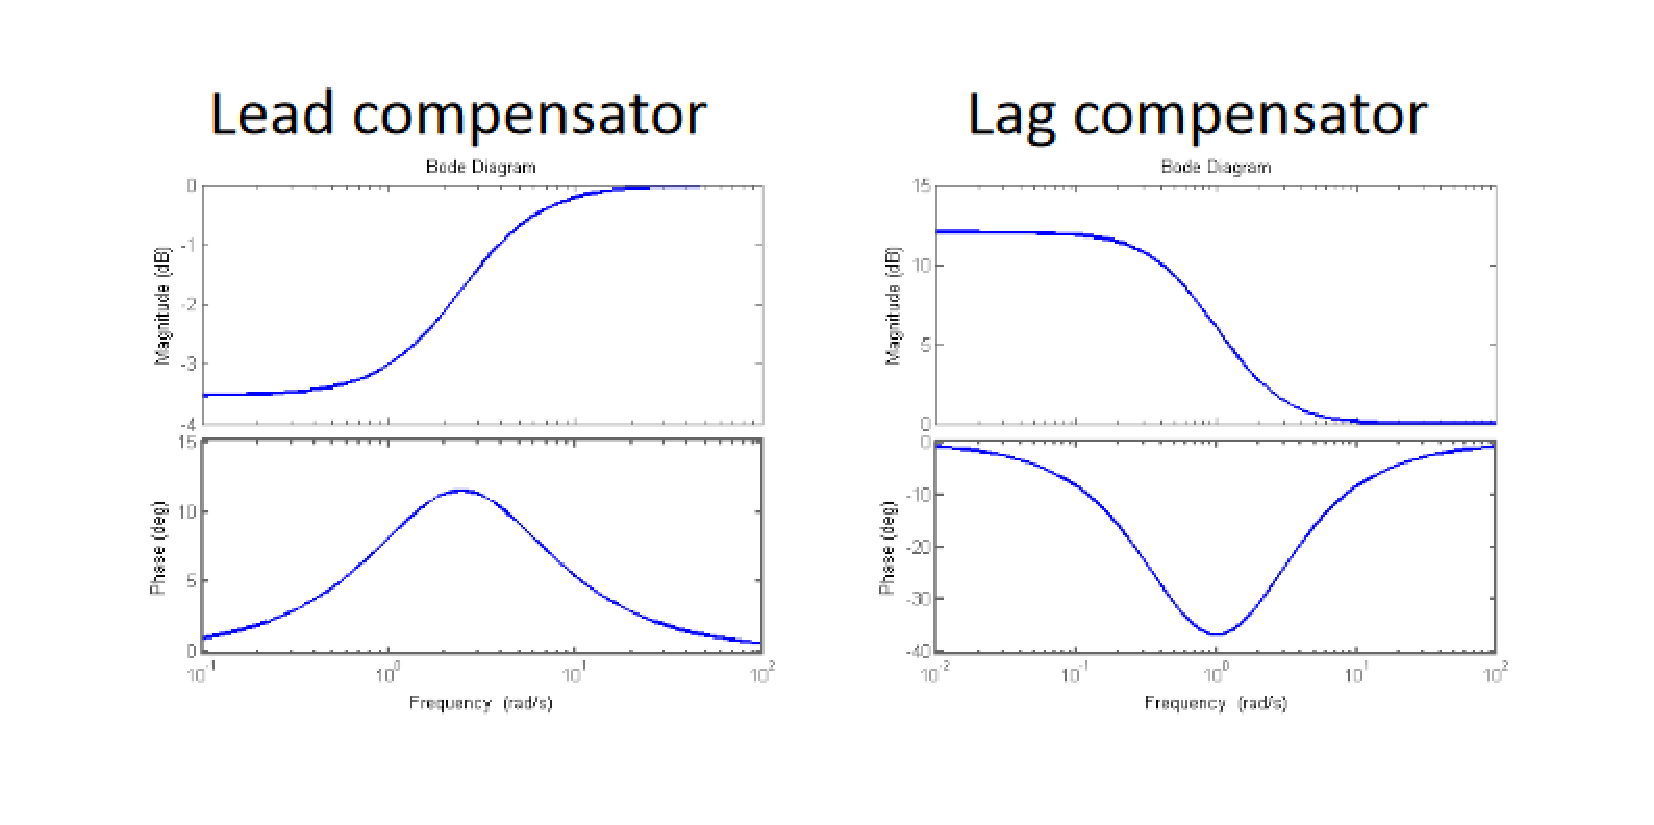
\includegraphics[width=1\linewidth, height=7cm ,inner]{./figs/ee18btech11027/Screen.eps} 
\label{fig:subim1}
\end{subfigure}
\end{figure}


\end{enumerate}
\end{document}